\documentclass[
    12pt,
    oneside,
    a4paper,
    brazil
]{abntex2}

\usepackage[utf8]{inputenc}
\usepackage[T1]{fontenc}
\usepackage[brazil]{babel}
\usepackage{graphicx}
\usepackage{booktabs}
\usepackage{float}
\usepackage{xltabular}
\usepackage{caption}
\usepackage{tabularx}
\usepackage{array}
\usepackage{svg}
\usepackage{tikz}
\usepackage{xcolor}

\newcolumntype{L}{>{\raggedright\arraybackslash}X}

\hypersetup{
    hidelinks
}

% --------------------------------------------------------

\begin{document}

% ---------------------------- CAPA ----------------------------

\begin{center}

\textbf{Grupo do Alef (e somente dele)} \\

Alef de Souza Lima - 10431891 \\
Gustavo Garabetti Munhoz - 10409258 \\
Renan Horochk de Andrade - 10438120 \\
Ryan Vinicius Ledo dos Santos - 10352727

\end{center}

\vfill

\begin{center}
    {\Large\textbf{Projeto - Laboratório de Engenharia de Software}}
\end{center}

\vfill

\begin{center}
    São Paulo \\
    2026/2
\end{center}

\newpage

% ---------------------------- SUMÁRIO ----------------------------

\tableofcontents*

\newpage

% --------------------------- CONTEÚDO ----------------------------

\textual

% --------------------------- INTRODUÇÃO ----------------------------

\chapter{Introdução}

A busca por oportunidades de trabalho nas periferias e bairros de menor renda enfrentam barreiras estruturais que vão além da escassez de postos formais de emprego. Nas comunidades periféricas, a dinamização da economia local ocorre principalmente por meio de relações de trabalho informais, prestação de serviços autônomos e pequenos comércios de bairro. No entanto, o avanço das tecnologias digitais de recrutamento não acompanhou a realidade dessas populações. As plataformas disponíveis atualmente no mercado priorizam vagas de caráter corporativo, exigem currículos estruturados e operam em escala metropolitana, ignorando a relevância dos pequenos "bicos" — como serviços de pintura, construção civil, aulas particulares de instrumentos musicais ou vagas operacionais em padarias, bares e pizzarias locais.

Essa desconexão entre a oferta de tecnologia e a realidade comunitária gera duas grandes distorções socioeconômicas. A primeira é o custo de deslocamento e de tempo, que inviabiliza que trabalhadores de menor renda aceitem oportunidades distantes de suas residências, uma vez que as despesas com transporte consomem grande parte do ganho obtido. A segunda é a competição predatória: a ausência de delimitação territorial nas plataformas convencionais faz com que profissionais de regiões mais abastadas ou distantes ocupem postos de trabalho em bairros periféricos, retirando da própria comunidade a oportunidade de suprir suas necessidades financeiras imediatas e de fazer a renda circular no próprio território.

Somado a esse cenário, a exclusão digital permanece como um obstáculo crítico. Uma parcela significativa do público de menor renda possui acesso limitado à internet móvel, planos de dados restritos ou baixa alfabetização digital, o que impede a utilização autônoma de ferramentas tecnológicas complexas. Dessa forma, os trabalhadores mais vulneráveis permanecem invisíveis tanto para o mercado formal quanto para as oportunidades do próprio bairro, dependendo exclusivamente do "boca a boca" ou de anúncios físicos precários espalhados pelas ruas.

Para intervir diretamente nessa problemática, este documento apresenta a especificação e o detalhamento de engenharia de uma aplicação web desenvolvida para essa finalidade. A solução proposta tem como propósito central aproximar contratantes locais e trabalhadores residentes no mesmo território, estabelecendo uma rede socioeconômica comunitária fundamentada na tecnologia. O grande vetor de inovação e o diferencial da plataforma residem no uso de um algoritmo de geolocalização restrita, que delimita rigorosamente a exibição de vagas e a candidatura a serviços a um raio máximo de até 5 km a partir da localização do usuário ou do estabelecimento. Essa restrição geográfica garante a retenção da renda na comunidade e prioriza o morador local no acesso às oportunidades da vizinhança.

Além disso, o software aborda frontalmente a exclusão digital ao introduzir o conceito de gestão intermediada. Através dessa funcionalidade, instituições parceiras estabelecidas nos bairros — como escolas públicas, ONGs e associações de moradores — atuam como sedes comunitárias de apoio. Essas entidades recebem credenciamento para cadastrar vagas de terceiros e realizar a inscrição no sistema em nome de cidadãos que não possuem dispositivos conectados ou que enfrentam dificuldades no manuseio de interfaces digitais.

Dessa forma, o projeto articula os princípios da Engenharia de Software — como modelagem de requisitos, arquitetura orientada a serviços e usabilidade voltada à acessibilidade — com uma forte demanda socioeconômica. O produto final visa ser um instrumento de inclusão produtiva, redução da desigualdade local e fortalecimento da economia dos bairros, servindo como uma ponte eficiente, segura e territorial entre quem precisa trabalhar e quem precisa contratar.

% --------------------------- DEMANDA ----------------------------

\chapter{Demanda}

\section{Oportunidade percebida}
Identificou-se uma lacuna no ecossistema de plataformas de empregos: a ausência de uma ferramenta voltada estritamente ao microcontexto territorial. As soluções existentes operam de escala metropolitana à internacional, o que expõe os trabalhadores locais de baixa renda a uma concorrência desigual com profissionais de regiões mais estruturadas ou distantes.

A oportunidade consiste em criar um canal exclusivo para o comércio local e para profissionais autônomos (pedreiros, pintores, eletricistas, professores particulares, entre outros) divulgarem e encontrarem serviços e vagas a uma curta distância de suas residências, retendo a renda dentro da própria comunidade.

\section{Razão para a demanda}
A demanda por essa solução fundamenta-se em três pilares socioeconômicos e tecnológicos principais:

\begin{itemize}
    \item \textbf{Mobilidade e Custo de Deslocamento}: Para trabalhadores de menor renda, o custo e o tempo de transporte público até regiões centrais comprometem significativamente o ganho líquido de trabalhos temporários ou de menor remuneração.
    \item \textbf{Inclusão Digital}: Uma parcela expressiva da população-alvo possui acesso limitado à internet ou baixa alfabetização digital, ficando à margem dos processos de seleção convencionais.
    \item \textbf{Proteção da Economia de Bairro}: A ausência de um filtro geográfico rígido faz com que oportunidades locais sejam absorvidas por pessoas de fora da comunidade, enfraquecendo a circulação financeira local.
\end{itemize}

\section{Descrição do software}
A plataforma consiste em uma aplicação web de intermediação de vagas e serviços informais pautada pela restrição geográfica. O sistema captura a localização do usuário ou do anúncio e restringe a exibição de oportunidades e candidaturas a um raio máximo de até 5 km. O sistema opera por meio de duas frentes principais: a publicação e candidatura direta feita por moradores e pequenos comerciantes, e a gestão intermediada. Nesta segunda frente, instituições parceiras credenciadas, como escolas públicas e ONGs, atuam como pontos de apoio físico para cadastrar oportunidades e inscrever cidadãos que não possuem acesso à internet ou facilidade com ferramentas digitais.

\section{Identificação dos usuários}
O sistema é estruturado em quatro perfis de acesso bem definidos. O Candidato ou Trabalhador Autônomo representa o morador que busca oportunidades informais ou divulga seus serviços na vizinhança. O Contratante Local engloba proprietários de pequenos estabelecimentos e moradores que necessitam de mão de obra pontual. A Sede Intermediadora compreende os agentes comunitários das entidades credenciadas, responsáveis por incluir digitalmente os cidadãos sem acesso. Por fim, o Administrador do Sistema é o encarregado da gestão de acessos, moderação de conteúdos e credenciamento das sedes parceiras.

\section{Etapas para construção do produto}
A condução do desenvolvimento do produto seguirá o ciclo de vida de engenharia de software estruturado nas seguintes etapas:

\begin{enumerate}
    \item \textbf{Elicitação e Análise de Requisitos:} Levantamento das necessidades dos usuários, mapeamento de regras de negócio (como o cálculo do raio de 5 km) e definição dos casos de uso.
    \item \textbf{Modelagem e Arquitetura:} Definição da arquitetura da aplicação web, modelagem do banco de dados e especificação das APIs de geolocalização.
    \item \textbf{Prototipação e Design de UX/UI:} Criação de protótipos de interface priorizando a acessibilidade, simplicidade visual e usabilidade para públicos com baixa alfabetização digital.
    \item \textbf{Desenvolvimento (Implementação):} Construção dos módulos de autenticação, controle de acesso baseado em papéis (RBAC), integração com serviços de mapas e geolocalização, e gestão de vagas.
    \item \textbf{Testes e Validação:} Execução de testes unitários, de integração, de usabilidade e testes de validação do filtro geográfico.
    \item \textbf{Implantação e Documentação:} Mapeamento de métricas, publicação da aplicação em ambiente de hospedagem e entrega da documentação técnica e de usuário.
\end{enumerate}

\section{Critérios de qualidade do produto}
Para garantir que a solução atenda adequadamente ao público-alvo e cumpra seus objetivos de engenharia, foram definidos os seguintes critérios de qualidade:

\begin{itemize}
    \item \textbf{Usabilidade e Acessibilidade:} Interface extremamente simples, intuitiva e adaptada para dispositivos móveis, minimizando a carga cognitiva para usuários com pouca familiaridade com tecnologia.
    \item \textbf{Precisão na Geolocalização:} Garantia de funcionamento rigoroso do algoritmo de filtragem por raio (até 5 km), impedindo a visualização e candidatura fora dos limites definidos.
    \item \textbf{Desempenho e Consumo de Dados:} Aplicação leve, otimizada para carregar rapidamente mesmo em conexões de internet móvel instáveis ou de baixa velocidade (3G/4G restrito).
    \item \textbf{Confiabilidade e Segurança:} Proteção dos dados pessoais dos trabalhadores e das instituições, garantindo que o cadastro intermediado por sedes mantenha a integridade das informações registradas.
\end{itemize}

% --------------------------- REQUISITOS ----------------------------

\chapter{Requisitos do produto}

\section{Requisitos funcionais}

\begin{xltabular}{\textwidth}{>{\raggedright\arraybackslash}p{1.2cm} >{\raggedright\arraybackslash}p{2.7cm} X >{\raggedleft\arraybackslash}p{2cm}}
    \label{tab:requisitos_func} \\
    \toprule
    \textbf{ID} & \textbf{Título} & \textbf{Descrição} & \textbf{Prioridade} \\
    \midrule
    \endfirsthead

    \multicolumn{4}{r}{} \\
    \toprule
    \textbf{ID} & \textbf{Título} & \textbf{Descrição} & \textbf{Prioridade} \\
    \midrule
    \endhead

    \midrule
    \endfoot

    \bottomrule
    \endlastfoot

    RF01 & Cadastro de Cidadãos & O sistema deve permitir o cadastro de moradores mediante o fornecimento de dados pessoais básicos, contatos e o endereço/localização de residência ou estabelecimento. & Alta \\ \hline
    RF02 & Gestão de Perfil do Cidadão & O sistema deve permitir que o morador realize a gestão de sua conta, incluindo a consulta, atualização de dados pessoais e de localização, bem como a solicitação de exclusão ou inativação do perfil. & Alta \\ \hline
    RF03 & Autenticação de Usuários & O sistema deve oferecer mecanismo de login seguro utilizando e-mail/CPF e senha para acesso às funcionalidades do sistema. & Alta \\ \hline
    RF04 & Cadastro de Sedes Intermediadoras & O sistema deve permitir que administradores cadastrem e credenciem entidades comunitárias parceiras (escolas, ONGs, associações) para atuarem como Sedes Intermediadoras. & Alta \\ \hline
    RF05 & Publicação e Divulgação de Oportunidades & O sistema deve permitir que os moradores publiquem ofertas de trabalho operacionais ou divulguem seus próprios serviços autônomos. & Alta \\ \hline
    RF06 & Gestão de Anúncios e Oportunidades & O sistema deve permitir que o autor do anúncio visualize, edite informações, altere o status (aberta, preenchida, cancelada) e exclua suas ofertas publicadas. & Alta \\ \hline
    RF07 & Candidatura e Contato Direto & O sistema deve permitir que o morador se aplique a uma vaga ou entre em contato direto com o anunciante através dos canais disponibilizados. & Alta \\ \hline
    RF08 & Filtragem por Geolocalização & O sistema deve calcular a distância entre a localização do morador e a vaga/serviço, exibindo exclusivamente as oportunidades localizadas dentro de um raio máximo de até 5 km. & Alta \\ \hline
    RF09 & Cadastro e Inscrição Intermediada & O sistema deve disponibilizar painel exclusivo para os agentes das Sedes Intermediadoras realizarem o cadastro e a candidatura de moradores sem acesso digital. & Alta \\ \hline
    RF10 & Gestão de Atendimento por Sedes & O sistema deve permitir que os agentes das Sedes Intermediadoras realizem a consulta, alteração de dados e cancelamento de cadastros ou candidaturas efetuados por elas. & Alta \\ \hline
    RF11 & Gestão das Sedes Intermediadoras & O sistema deve permitir aos administradores a atualização de dados, consulta e revogação/descredenciamento do acesso de Sedes Intermediadoras. & Média \\ \hline
    RF12 & Exibição em Lista Ordenada & O sistema deve permitir a visualização das oportunidades e serviços em formato de lista ordenada por proximidade geográfica. & Média \\
\end{xltabular}

\section{Requisitos não-funcionais}
\begin{xltabular}{\textwidth}{>{\raggedright\arraybackslash}p{1.2cm} >{\raggedright\arraybackslash}p{2.7cm} X >{\raggedleft\arraybackslash}p{2cm}}
    \label{tab:requisitos_nao_func} \\

    \toprule
    \textbf{ID} & \textbf{Título} & \textbf{Descrição} & \textbf{Prioridade} \\
    \midrule
    \endfirsthead

    \multicolumn{4}{r}{} \\
    \toprule
    \textbf{ID} & \textbf{Título} & \textbf{Descrição} & \textbf{Prioridade} \\
    \midrule
    \endhead

    \midrule
    \endfoot

    \bottomrule
    \endlastfoot

    RNF01 & Tempo de Resposta & O cálculo da distância por geolocalização e o carregamento do feed de vagas devem ser executados em um tempo inferior a 2 segundos em condições normais de conexão & Alta \\ \hline
    RNF02 & Usabilidade e Baixa Carga Cognitiva & A interface de usuário deve adotar conceitos de acessibilidade e simplicidade visual, utilizando linguagem clara, ícones intuitivos e poucos cliques para concluir ações principais, atendendo a usuários com baixa alfabetização digital & Alta \\ \hline
    RNF03 & Proteção de Dados Pessoais (LGPD) & O sistema deve tratar os dados pessoais e de localização dos usuários em conformidade com a Lei Geral de Proteção de Dados, garantindo criptografia em trânsito (protocolo HTTPS) e consentimento explícito para captura da posição geográfica & Alta \\ \hline
    RNF04 & Controle de Acesso Baseado em Papéis (RBAC) & O sistema deve isolar estritamente as permissões de cada tipo de perfil (Candidato, Contratante, Sede Intermediadora e Administrador), impedindo acesso não autorizado a dados sensíveis de terceiros & Alta \\ \hline
    RNF05 & Disponibilidade & O sistema deve manter um índice de disponibilidade (uptime) mínimo de 99\% em ambiente de produção. & Média \\ \hline
    RNF06 & Escalabilidade & A arquitetura do sistema deve ser preparada para suportar o aumento do número de requisições simultâneas conforme novas regiões ou sedes comunitárias forem adicionadas à plataforma & Média \\ \hline
    RNF07 & Desempenho e Consumo de Dados & O sistema deve ser leve e otimizado para carregamento rápido em redes de internet móvel instáveis ou de baixa velocidade, limitando o peso das páginas iniciais e recursos de mídia. & Média \\ \hline
    RNF08 & Design Responsivo & A aplicação web deve ser totalmente adaptável a telas de smartphones de pequeno e médio porte, visto que o público-alvo pode acessá-lo também localmente, sem ir a uma sede intermediadora & Média \\ \hline

\end{xltabular}

% --------------------------- WIREFRAMES ----------------------------

\chapter{Wireframes}

\section{Caso de uso UC01 -- Registrar vaga}
O representante acessa a página de cadastro de vagas. Nessa página, ele irá inserir os dados e detalhes da oportunidade (título, descrição, período, salário, benefícios, requisitos e modalidade de trabalho) e clicar no botão de confirmação.

\section{Caso de uso UC02 -- Candidatar-se à vaga}
O Candidato acessa a página de vagas. Nessa página, ele irá selecionar uma vaga de interesse e se candidatar a ela.

\begin{figure}[H]
    \centering
    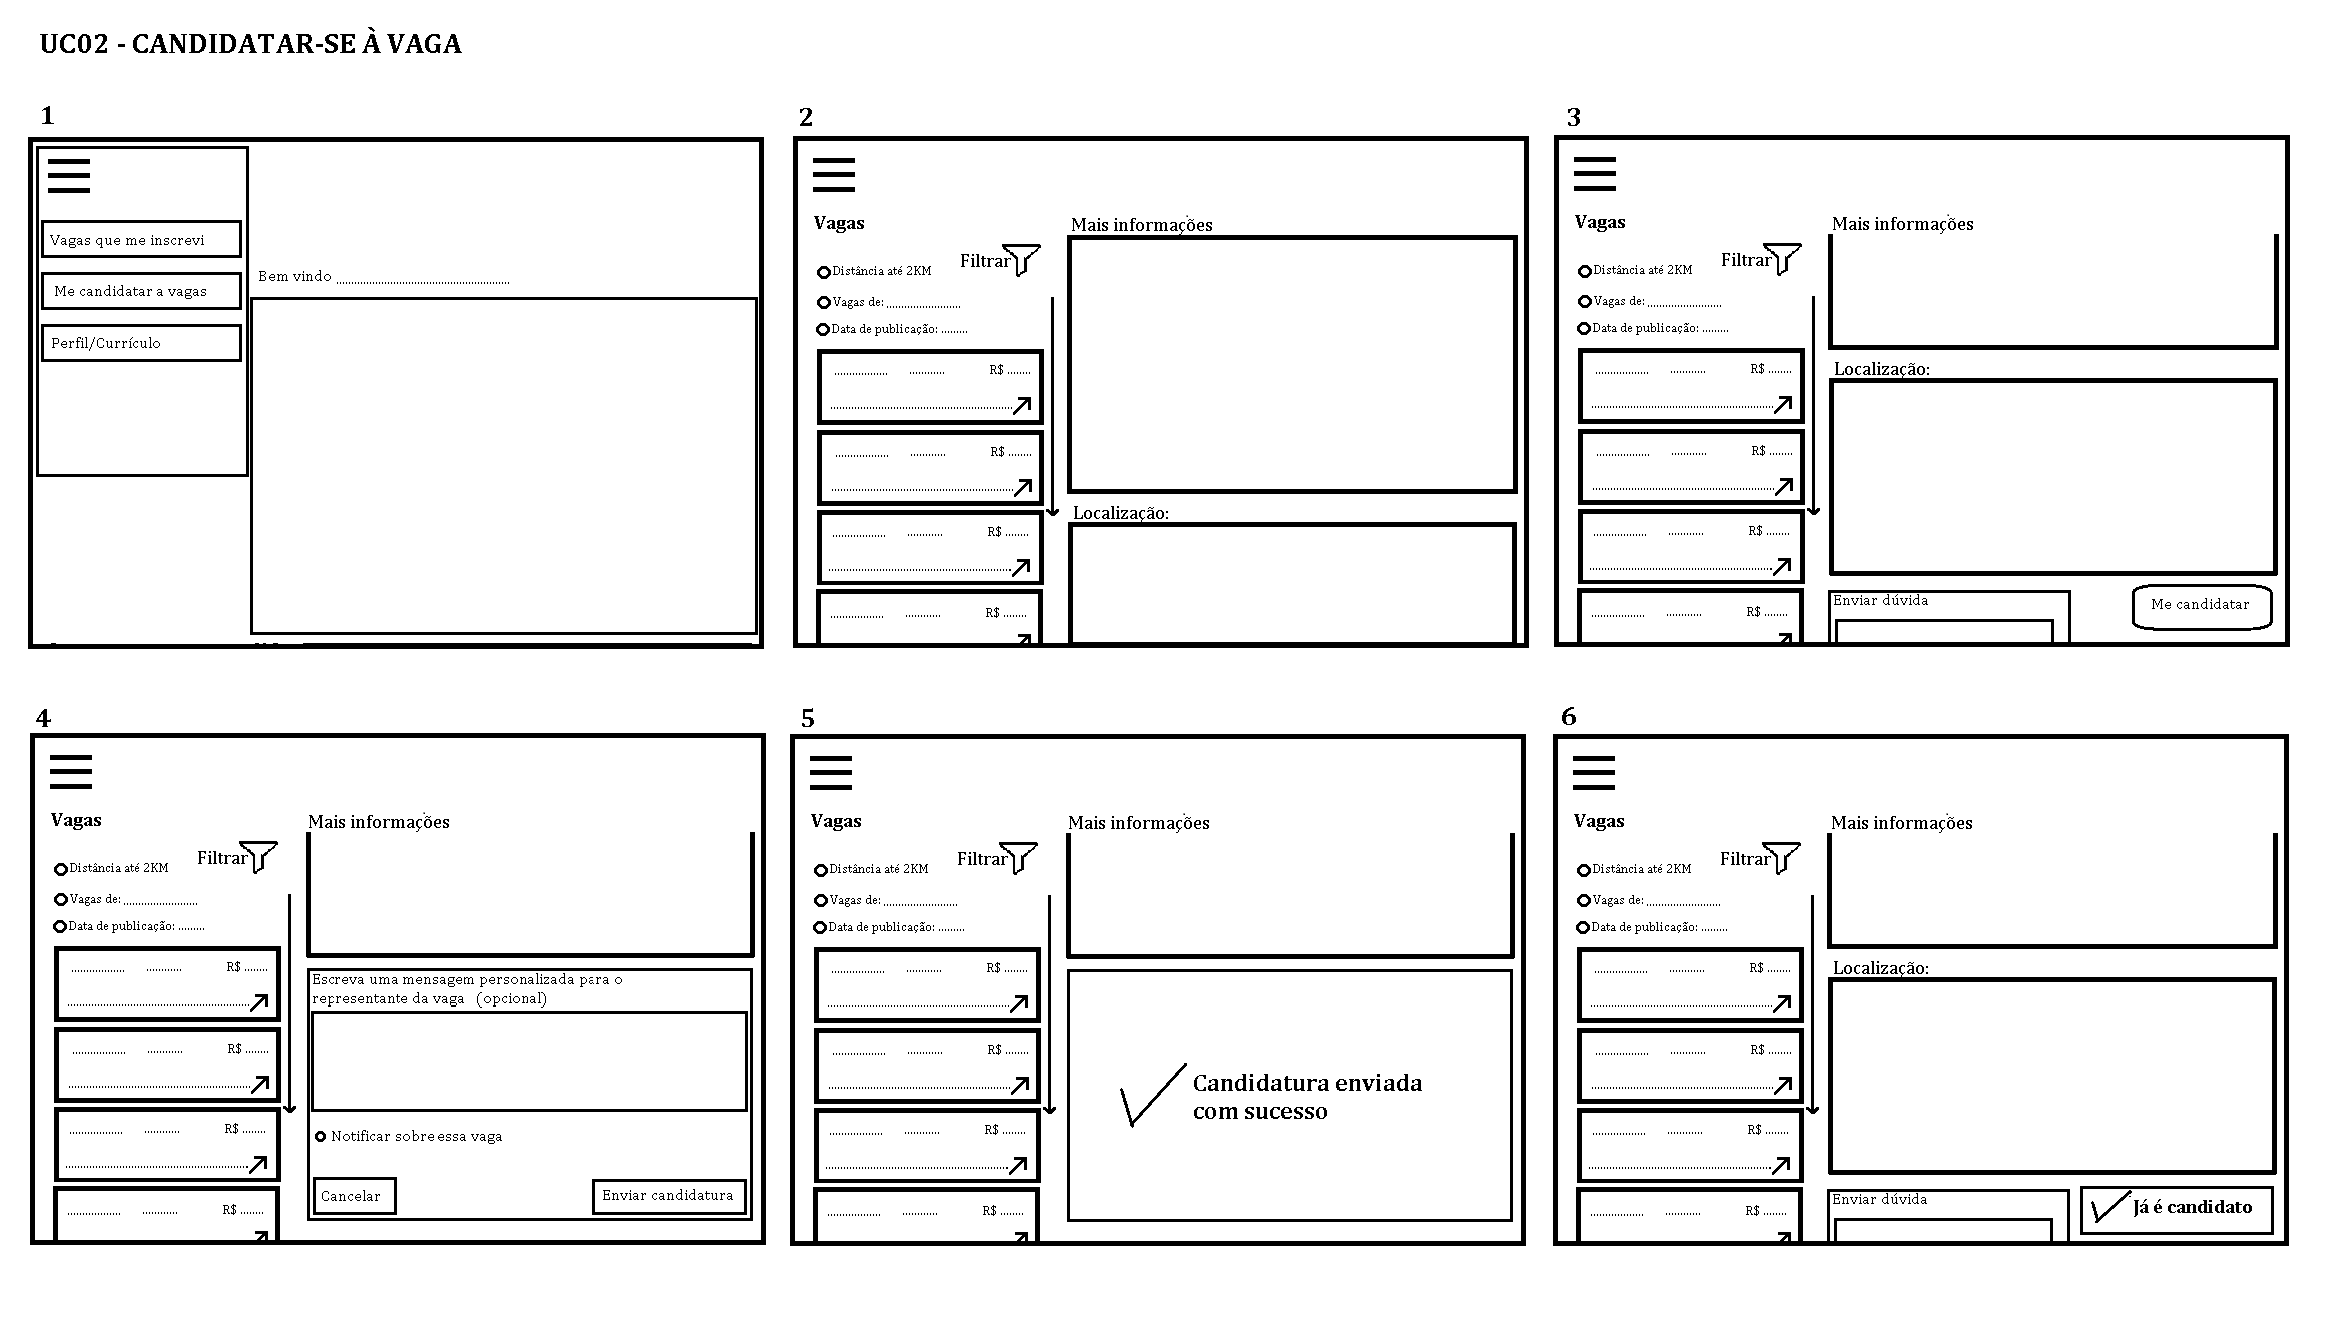
\includegraphics[width=0.85\linewidth]{UC02_candidatar_se_a_vaga.png}
    \caption{Wireframe do caso de uso UC02: Candidatar-se à vaga.}
    \label{fig:wireframe_uc02}
\end{figure}

% --------------------------- MODELAGEM ----------------------------

\chapter{Modelagem do sistema}

\section{Diagrama de Casos de Uso}
A Figura~\ref{fig:Diagram_Caso} ilustra os casos de uso mapeados para a plataforma comunitária, detalhando as interações do colaborador/candidato, do intermediário comunitário e das oportunidades.

\begin{figure}[H]
    \centering
    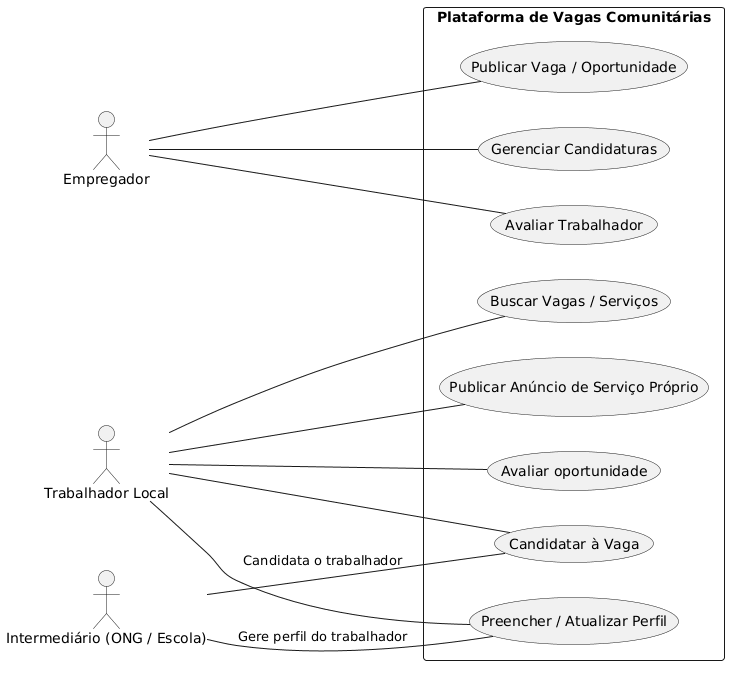
\includegraphics[width=0.8\linewidth]{use-case-diagram.png}
    \caption{Diagrama de Casos de Uso da Plataforma de Vagas Comunitárias.}
    \label{fig:Diagram_Caso}
\end{figure}

\section{Modelo de Domínio}
A Figura~\ref{fig:diagrama_dominio} apresenta o modelo conceitual de domínio da aplicação, com suas entidades centrais e relacionamentos.

\begin{figure}[H]
    \centering
    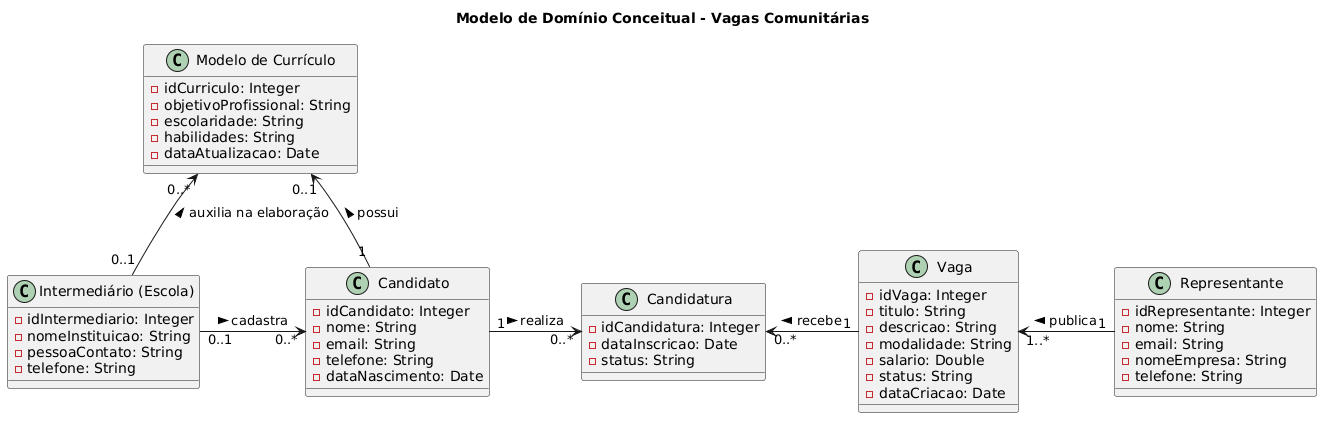
\includegraphics[width=1\linewidth]{Diagram_Dominioteste.png}
    \caption{Diagrama de Domínio Conceitual do Sistema.}
    \label{fig:diagrama_dominio}
\end{figure}

\section{Especificação dos Casos de Uso}

% --- UC01 ---
\subsection{UC01 -- Publicar Vagas Locais}

\begin{figure}[H]
    \centering
    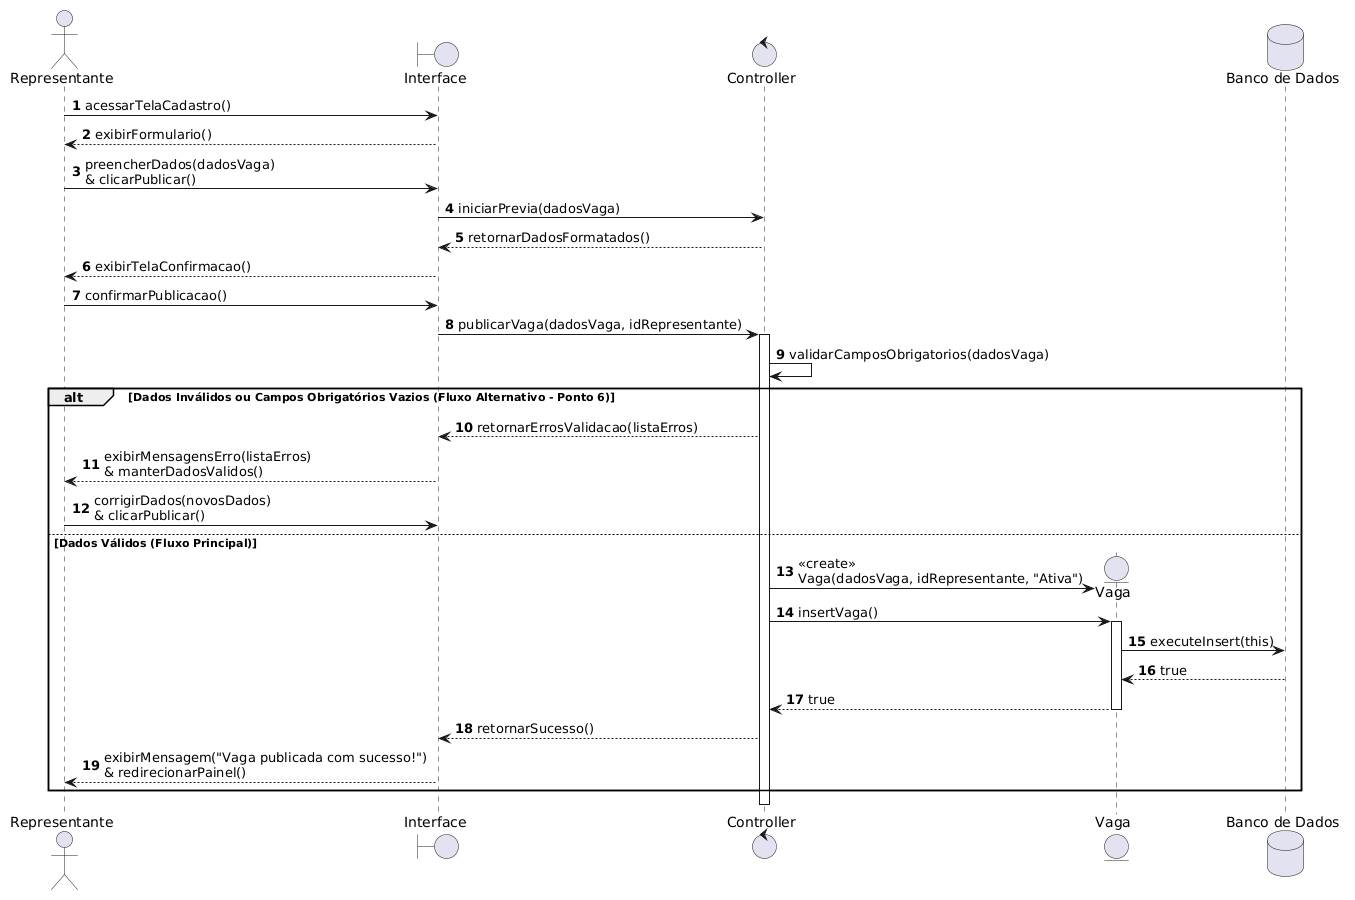
\includegraphics[width=1\linewidth]{Diagrama_sequ_UC01.png}
    \caption{Diagrama de Sequência referente ao Caso de Uso UC01.}
    \label{fig:seq_uc01}
\end{figure}

\begin{table}[H]
\centering
\small
\begin{tabularx}{\textwidth}{@{}>{\bfseries}p{3.5cm} L@{}}
\toprule
Identificador & UC01 \\
\midrule
Nome & Publicar Vagas Locais \\
\midrule
Atores & Candidato/Representante \\
\midrule
Sumário & O representante acessa a página de cadastro de vagas. Nessa página, ele irá inserir os dados e detalhes da oportunidade (título, descrição, período, salário, benefícios, requisitos e modalidade de trabalho) e clicar no botão de confirmação. \\
\midrule
Pré-condição & O representante deve estar logado. \\
\midrule
Pós-condição & A vaga é registrada no banco de dados com status 'Ativa' (disponível para consulta dos candidatos) e uma mensagem de sucesso é exibida ao representante. \\
\midrule
Pontos de Inclusão & -- \\
\midrule
Pontos de Extensão & -- \\
\bottomrule
\end{tabularx}
\caption{Especificação do Caso de Uso UC01.}
\label{tab:uc01_espec}
\end{table}

\paragraph{Fluxo Principal}
\begin{table}[H]
\centering
\small
\begin{tabularx}{\textwidth}{@{}>{\bfseries}p{1.2cm} L L@{}}
\toprule
Passo & Ações do Ator & Ações do Sistema \\
\midrule
1 & O representante acessa a página de cadastro de vagas. & -- \\
2 & -- & O sistema apresenta o formulário de cadastro com os campos necessários para o preenchimento da vaga. \\
3 & O representante preenche os dados solicitados e seleciona a opção ``Publicar Vaga''. & -- \\
4 & -- & O sistema apresenta uma tela para confirmação das informações preenchidas. \\
5 & O representante confere os dados e seleciona o botão ``Confirmar Vaga''. & -- \\
6 & -- & O sistema valida se todos os campos obrigatórios foram preenchidos e se as informações estão de acordo com os critérios definidos. \\
7 & -- & O sistema registra a vaga na base de dados, vinculando-a ao ID do representante e registrando a data de criação e o status ``Ativa''. \\
8 & -- & O sistema exibe a mensagem ``Vaga publicada com sucesso!'' e redireciona o representante para a tela de detalhes ou para a listagem de suas vagas. \\
\bottomrule
\end{tabularx}
\caption{Fluxo Principal do UC01.}
\label{tab:uc01_fluxo_principal}
\end{table}

\paragraph{Fluxo Alternativo -- Ponto 6: Dados Inválidos ou Campos Obrigatórios Vazios}
\begin{itemize}
    \item \textbf{7.} O sistema identifica que existem campos obrigatórios não preenchidos ou informações que não atendem aos critérios de validação, como título em branco, salário em formato inválido ou descrição ausente.
    \item \textbf{8.} O sistema exibe mensagens de erro próximas aos campos que apresentam inconsistências, indicando o que precisa ser corrigido.
    \item \textbf{9.} O sistema mantém as informações válidas já preenchidas no formulário.
    \item \textbf{10.} O representante corrige as informações e tenta publicar a vaga novamente.
    \item \textbf{11.} O sistema retoma o processo a partir do passo 3 do Fluxo Principal.
\end{itemize}

\vspace{0.5cm}

% --- UC02 ---
\subsection{UC02 -- Candidatar-se à Vaga}

\begin{figure}[H]
    \centering
    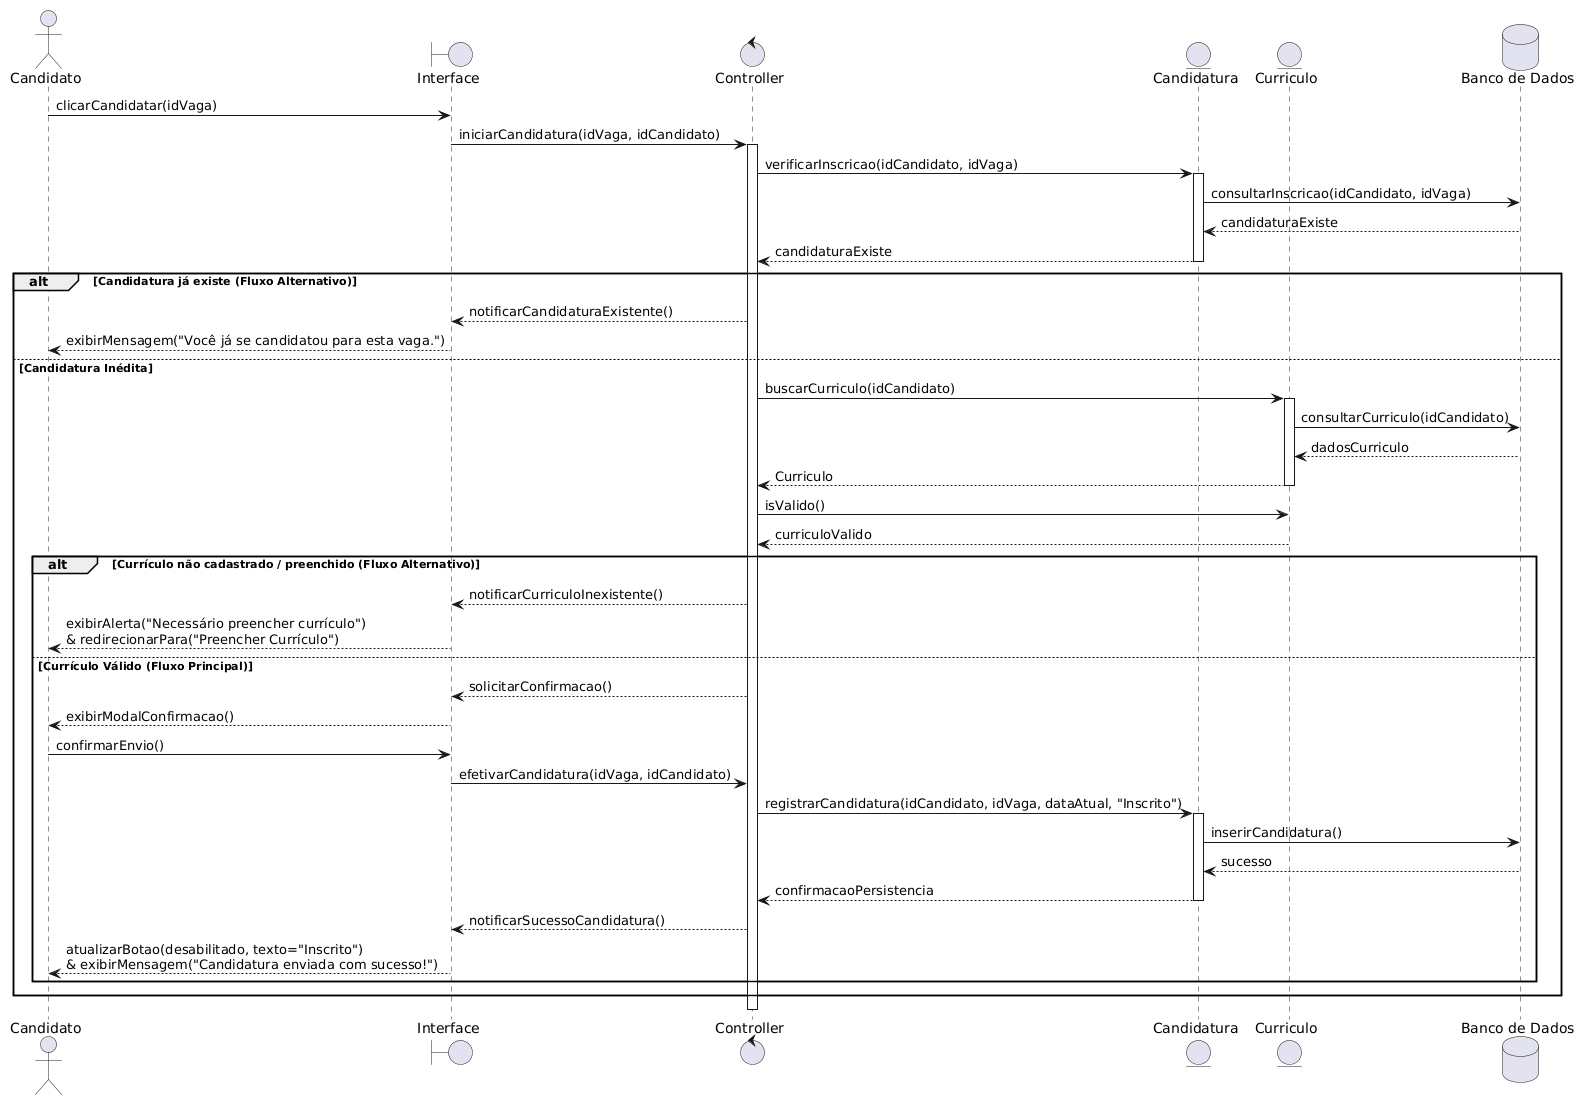
\includegraphics[width=1\linewidth]{Diagrama_sequ_UC02.png}
    \caption{Diagrama de Sequência referente ao Caso de Uso UC02.}
    \label{fig:seq_uc02}
\end{figure}

\begin{table}[H]
\centering
\small
\begin{tabularx}{\textwidth}{@{}>{\bfseries}p{3.5cm} L@{}}
\toprule
Identificador & UC02 \\
\midrule
Nome & Candidatar-se à Vaga \\
\midrule
Atores & Candidato/Representante \\
\midrule
Sumário & O Candidato acessa a página de vagas. Nessa página, ele irá selecionar uma vaga de interesse e se candidatar a ela. \\
\midrule
Pré-condição & O Candidato deve estar logado e possuir um currículo cadastrado. \\
\midrule
Pós-condição & A candidatura é registrada com sucesso no sistema, atualizando o status da vaga para ``Inscrito'' no painel do candidato e disponibilizando seu perfil para o recrutador. \\
\midrule
Pontos de Inclusão & -- \\
\midrule
Pontos de Extensão & -- \\
\bottomrule
\end{tabularx}
\caption{Especificação do Caso de Uso UC02.}
\label{tab:uc02_espec}
\end{table}

\paragraph{Fluxo Principal}
\begin{table}[H]
\centering
\small
\begin{tabularx}{\textwidth}{@{}>{\bfseries}p{1.2cm} L L@{}}
\toprule
Passo & Ações do Ator & Ações do Sistema \\
\midrule
1 & O candidato ou representante seleciona a opção ``Candidatar-se'' na página da vaga desejada. & -- \\
2 & -- & O sistema verifica se o usuário possui uma sessão ativa e se há um currículo cadastrado. \\
3 & -- & O sistema verifica se o candidato já realizou uma candidatura para a vaga selecionada. \\
4 & -- & O sistema apresenta uma janela solicitando a confirmação da candidatura. \\
5 & O candidato confirma o envio da candidatura. & -- \\
6 & -- & O sistema registra a candidatura, associando o candidato à vaga, a data do envio e o status ``Inscrito''. \\
7 & -- & O sistema atualiza a página da vaga, deixando o botão de candidatura desabilitado e alterando seu texto para ``Inscrito''. \\
8 & -- & O sistema exibe a mensagem ``Candidatura enviada com sucesso!''. \\
\bottomrule
\end{tabularx}
\caption{Fluxo Principal do UC02.}
\label{tab:uc02_fluxo_principal}
\end{table}

\paragraph{Fluxo Alternativo -- Ponto 2: Currículo não preenchido}
\begin{itemize}
    \item \textbf{3.} O sistema identifica que o candidato não possui um currículo cadastrado.
    \item \textbf{4.} O sistema exibe um alerta informando que é necessário possuir um currículo preenchido para realizar a candidatura.
    \item \textbf{5.} O sistema redireciona o candidato para a tela do caso de uso ``Preencher Currículo''.
    \item \textbf{6.} O candidato preenche o currículo e retorna ao processo de candidatura.
    \item \textbf{7.} O sistema direciona o candidato novamente para o passo 1 do Fluxo Principal.
\end{itemize}

\paragraph{Fluxo Alternativo -- Ponto 3: Candidatura já existe}
\begin{itemize}
    \item \textbf{4.} O sistema identifica que o candidato já possui uma candidatura ativa para a vaga selecionada.
    \item \textbf{5.} O sistema exibe uma mensagem informando: ``Você já se candidatou para esta vaga.''
\end{itemize}

\vspace{0.5cm}

% --- UC03 ---
\subsection{UC03 -- Preencher Currículo}

\begin{figure}[H]
    \centering
    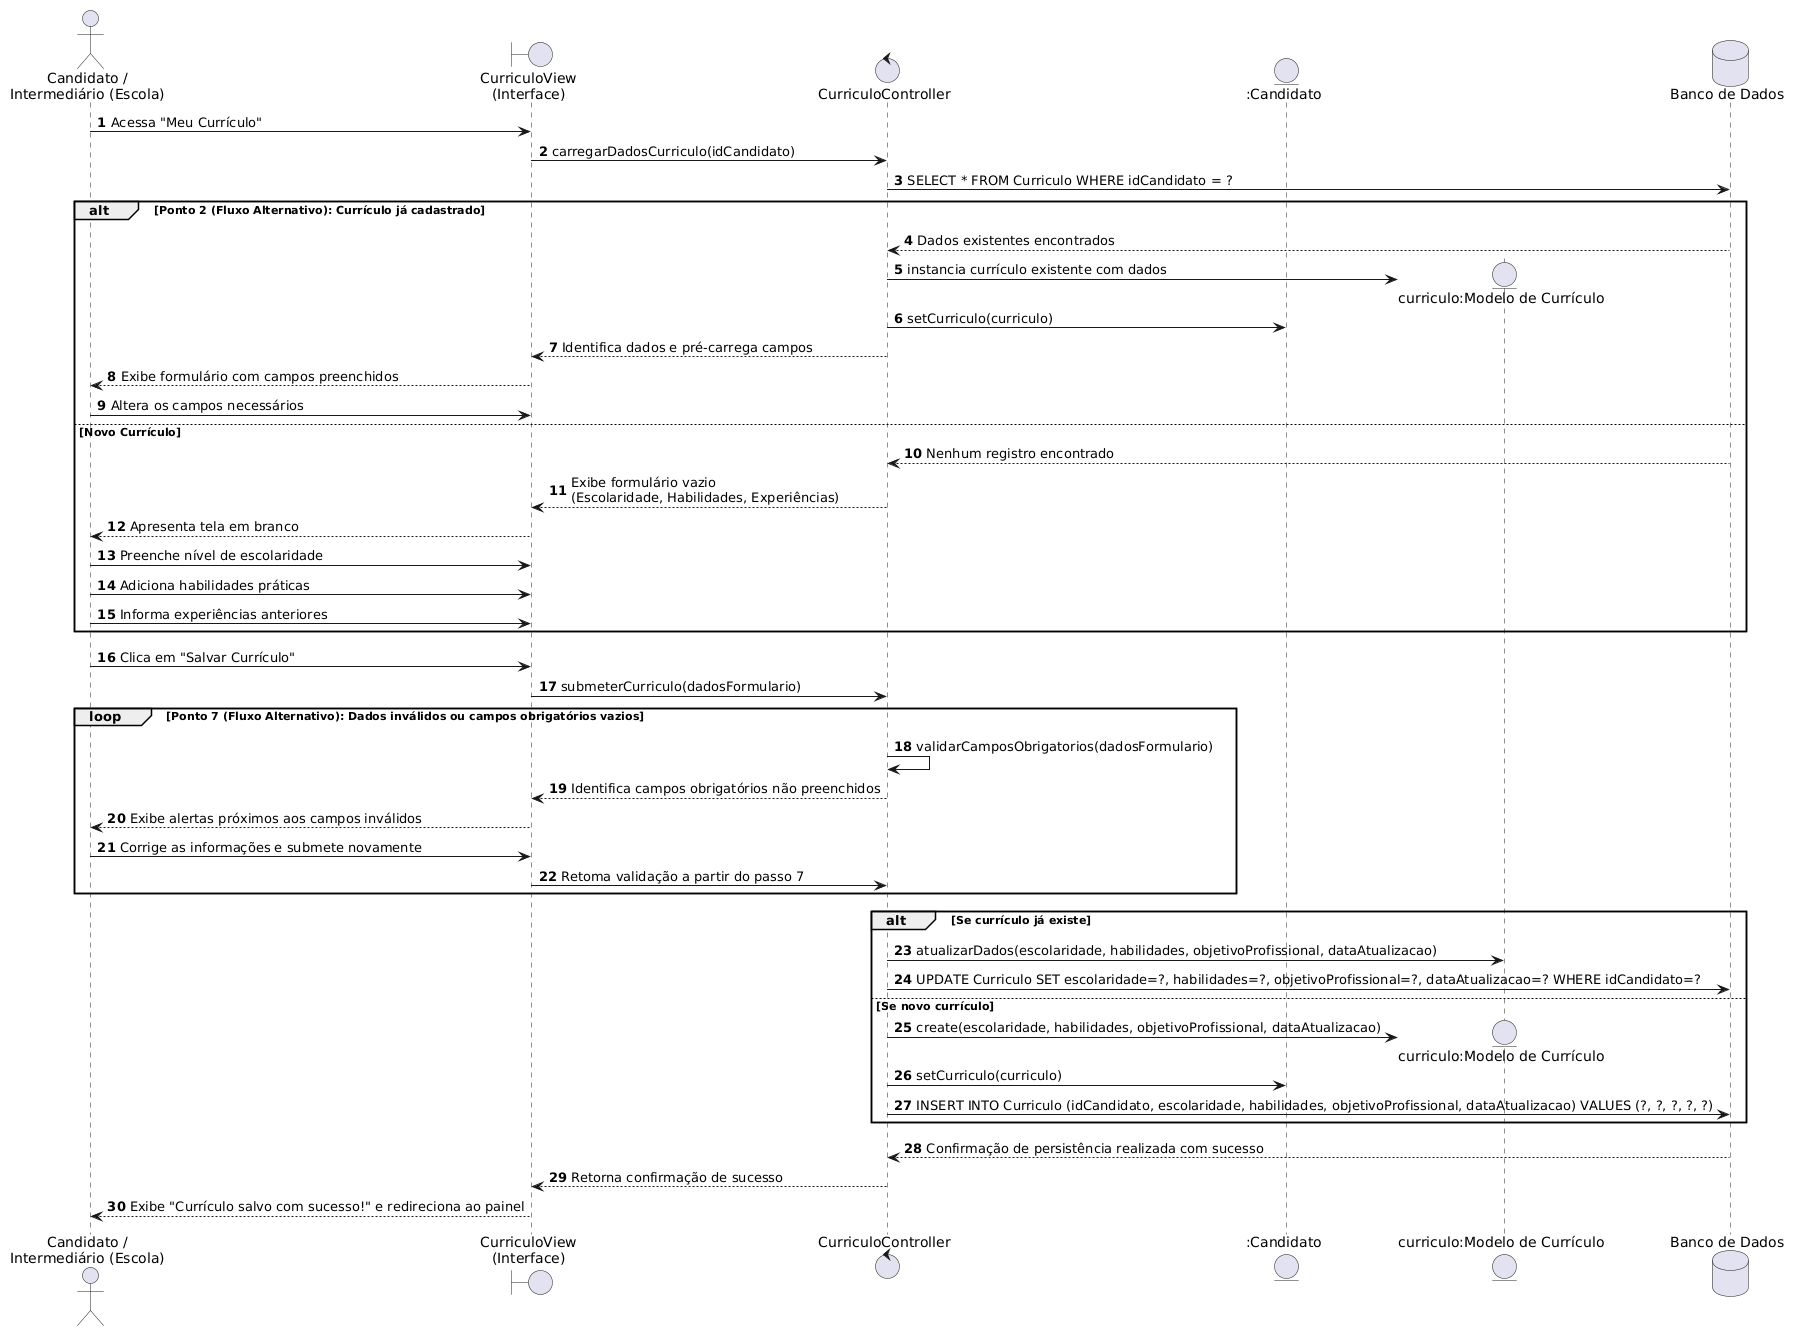
\includegraphics[width=1\linewidth]{Diagrama_sequ_UC03.png}
    \caption{Diagrama de sequência referente ao Caso de Uso UC03.}
    \label{fig:Diagrama_sequ_UC03}
\end{figure}

\begin{table}[H]
\centering
\small
\begin{tabularx}{\textwidth}{@{}>{\bfseries}p{3.5cm} L@{}}
\toprule
Identificador & UC03 \\
\midrule
Nome & Preencher Currículo \\
\midrule
Atores & Colaborador, Intermediário (Escola) \\
\midrule
Sumário & O usuário acessa a seção de perfil/currículo para registrar ou atualizar suas informações profissionais, incluindo formação acadêmica/escolaridade, histórico de experiências e habilidades práticas, disponibilizando esses dados para futuras candidaturas. \\
\midrule
Pré-condição & O usuário (Colaborador ou Intermediário representando o cidadão) deve estar autenticado no sistema. \\
\midrule
Pós-condição & As informações do currículo são persistidas no banco de dados vinculadas ao perfil do cidadão, tornando-o apto a se candidatar às vagas da plataforma. \\
\midrule
Pontos de Inclusão & -- \\
\midrule
Pontos de Extensão & -- \\
\bottomrule
\end{tabularx}
\caption{Especificação do Caso de Uso UC03.}
\label{tab:uc03_espec}
\end{table}

\paragraph{Fluxo Principal}
\begin{table}[H]
\centering
\small
\begin{tabularx}{\textwidth}{@{}>{\bfseries}p{1.2cm} L L@{}}
\toprule
Passo & Ações do Ator & Ações do Sistema \\
\midrule
1 & O usuário acessa a opção ``Meu Currículo'' no menu principal. & -- \\
2 & -- & O sistema carrega e exibe o formulário de currículo dividido em seções: Nível de escolaridade, Habilidades e Experiências. \\
3 & O usuário preenche o nível de escolaridade. & -- \\
4 & O usuário adiciona uma ou mais habilidades práticas. & -- \\
5 & O usuário informa suas experiências anteriores (locais, períodos e descrição). & -- \\
6 & O usuário seleciona a opção ``Salvar Currículo''. & -- \\
7 & -- & O sistema valida se as informações obrigatórias foram preenchidas. \\
8 & -- & O sistema salva os dados do currículo vinculados ao ID do colaborador. \\
9 & -- & O sistema exibe a mensagem ``Currículo salvo com sucesso!'' e redireciona para o painel principal. \\
\bottomrule
\end{tabularx}
\caption{Fluxo Principal do UC03.}
\label{tab:uc03_fluxo_principal}
\end{table}

\paragraph{Fluxo Alternativo -- Ponto 2: Currículo já preenchido}
\begin{itemize}
    \item \textbf{3.} O sistema identifica dados salvos previamente e pré-carrega os campos.
    \item \textbf{4.} O usuário realiza alteração nos campos necessários e retorna ao passo 6 do Fluxo Principal.
\end{itemize}

\paragraph{Fluxo Alternativo -- Ponto 7: Dados inválidos ou campos obrigatórios vazios}
\begin{itemize}
    \item \textbf{8.} O sistema identifica que existem campos obrigatórios não preenchidos ou dados inconsistentes.
    \item \textbf{9.} O sistema exibe mensagens de erro próximas aos campos que apresentam inconsistências, indicando o que precisa ser corrigido.
    \item \textbf{10.} O usuário corrige as pendências e seleciona a opção ``Salvar Currículo'' novamente.
    \item \textbf{11.} O sistema retoma a validação a partir do passo 7 do Fluxo Principal.
\end{itemize}

% --------------------------- ARQUITETURA ----------------------------
\chapter{Arquitetura do sistema}

A plataforma é estruturada em uma arquitetura orientada a serviços, composta por um frontend web, um gateway de entrada e dois serviços de backend independentes, todos hospedados na Amazon Web Services (AWS). A comunicação entre o cliente e a infraestrutura ocorre exclusivamente por meio do protocolo HTTPS, garantindo a criptografia dos dados em trânsito, conforme exigido pelo requisito RNF03.

A Figura~\ref{fig:arquitetura-sistema} apresenta o diagrama de implantação da arquitetura do sistema.

\begin{figure}[H]
\centering
\resizebox{\textwidth}{!}{%
\begin{tikzpicture}[
    font=\small,
    arr/.style={->, >=stealth, thick, black}
]

% ── Nós externos: clientes ────────────────────────────────────────────
\draw[thick] (0, 7.5) rectangle (3.5, 9.0);
\node[anchor=north west, font=\scriptsize] at (0.1, 9.0) {«node»};
\node[font=\small, align=center] at (1.75, 8.1) {cliente:\\Browser};

\draw[thick] (0, 5.5) rectangle (3.5, 7.0);
\node[anchor=north west, font=\scriptsize] at (0.1, 7.0) {«node»};
\node[font=\small, align=center] at (1.75, 6.1) {cliente:\\Smartphone};

% ── Nó externo: Ambiente AWS ──────────────────────────────────────────
\draw[thick] (4.5, 0.0) rectangle (18.0, 11.2);
\node[anchor=north west, font=\scriptsize] at (4.6, 11.2) {«node»};
\node[anchor=north west, font=\small\bfseries] at (5.2, 10.8) {Ambiente AWS};

    % ── Nó: API Gateway ───────────────────────────────────────────────
    \draw[thick] (5.0, 7.5) rectangle (10.5, 9.5);
    \node[anchor=north west, font=\scriptsize] at (5.1, 9.5) {«node» gateway: Amazon API Gateway};
    \draw[thick] (5.4, 7.8) rectangle (10.1, 9.0);
    \node[anchor=north west, font=\scriptsize] at (5.5, 9.0) {«artifact»};
    \node[font=\small, align=center] at (7.75, 8.3) {Amazon API Gateway};

    % ── Nó: Frontend EC2 ──────────────────────────────────────────────
    \draw[thick] (11.5, 7.5) rectangle (17.5, 9.5);
    \node[anchor=north west, font=\scriptsize] at (11.6, 9.5) {«node» frontend: Amazon EC2};
    \draw[thick] (11.9, 7.8) rectangle (17.1, 9.0);
    \node[anchor=north west, font=\scriptsize] at (12.0, 9.0) {«artifact»};
    \node[font=\small, align=center] at (14.5, 8.3) {Nginx + React (SPA)};

    % ── Nó: EC2 Serviços ──────────────────────────────────────────────
    \draw[thick] (5.0, 0.5) rectangle (10.5, 7.0);
    \node[anchor=north west, font=\scriptsize] at (5.1, 7.0) {«node» app: Amazon EC2};

        % Serviço de Usuários
        \draw[thick] (5.4, 4.2) rectangle (10.1, 6.4);
        \node[anchor=north west, font=\scriptsize] at (5.5, 6.4) {«artifact»};
        \node[font=\small, align=center] at (7.75, 5.2) {Serviço de\\Usuários};

        % Serviço de Oportunidades
        \draw[thick] (5.4, 1.0) rectangle (10.1, 3.8);
        \node[anchor=north west, font=\scriptsize] at (5.5, 3.8) {«artifact»};
        \node[font=\small, align=center] at (7.75, 2.3) {Serviço de\\Oportunidades};

    % ── Nó: Aurora ────────────────────────────────────────────────────
    \draw[thick] (11.5, 0.5) rectangle (17.5, 7.0);
    \node[anchor=north west, font=\scriptsize] at (11.6, 7.0) {«node» db: Amazon Aurora};
    \draw[thick] (11.9, 1.0) rectangle (17.1, 6.5);
    \node[anchor=north west, font=\scriptsize] at (12.0, 6.5) {«database»};
    \node[font=\small, align=center] at (14.5, 3.6) {Aurora PostgreSQL};

% ── Setas ─────────────────────────────────────────────────────────────

% clientes → Frontend
\draw[arr] (3.5, 8.25) -- (11.5, 8.8);
\draw[arr] (3.5, 6.25) -- (11.5, 8.0);

% Frontend → API Gateway
\draw[arr] (11.5, 8.5) -- (10.5, 8.5);

% API Gateway → EC2 Serviços
\draw[arr] (7.75, 7.5) -- (7.75, 6.4);

% Oportunidades → Usuários
\draw[arr] (7.75, 3.8) -- (7.75, 4.2);

% Serviços → Aurora
\draw[arr] (10.1, 5.3) -- (11.9, 4.5);
\draw[arr] (10.1, 2.4) -- (11.9, 2.8);

\end{tikzpicture}%
}
\caption{Diagrama de implantação da arquitetura do sistema.}
\label{fig:arquitetura-sistema}
\end{figure}

\begin{figure}[H]
    \centering
    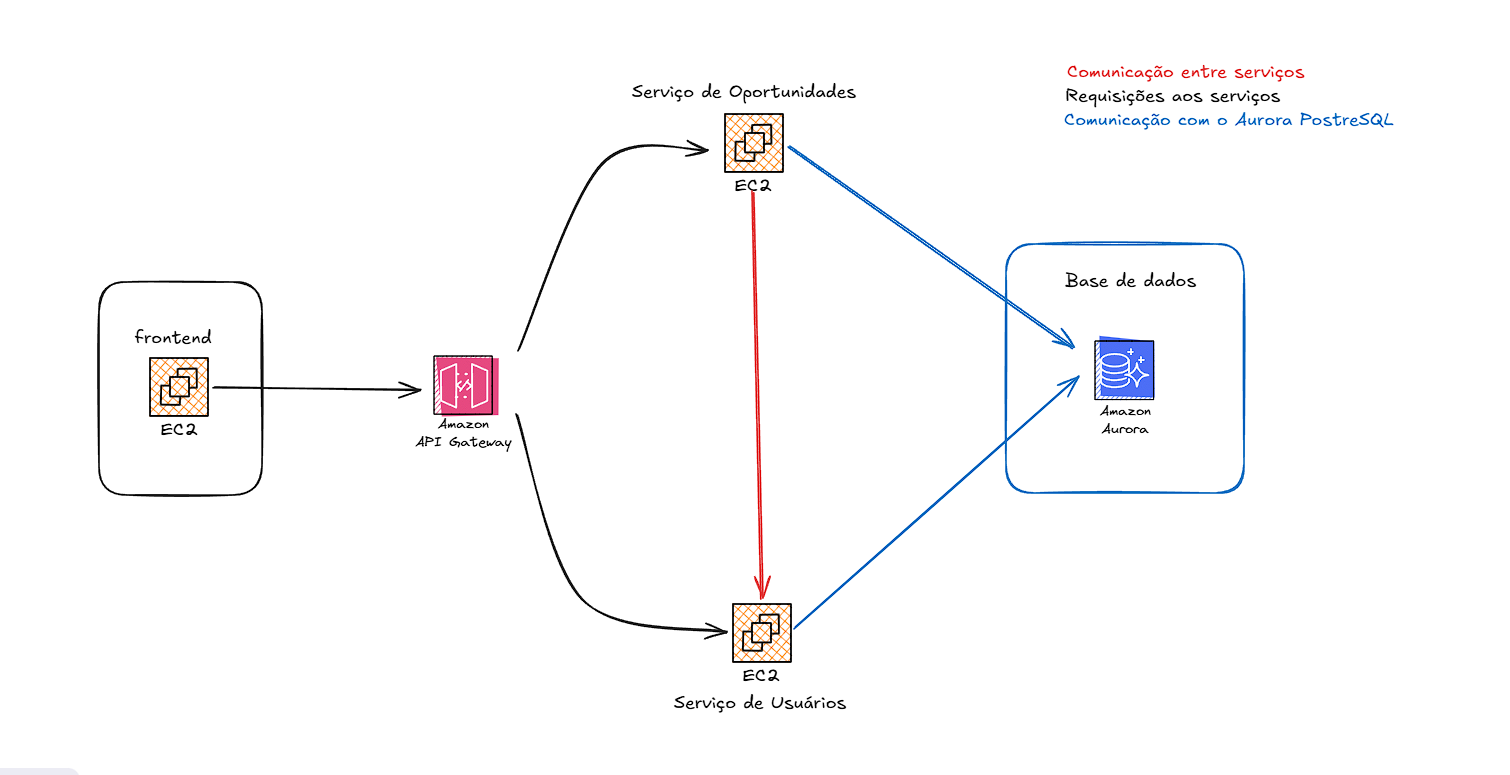
\includegraphics[width=1\linewidth]{image.png}
    \caption{Desenho da arquitetura}
    \label{fig:placeholder}
\end{figure}

\section{Componentes principais}

A arquitetura é composta pelos seguintes componentes:

\begin{itemize}
    \item \textbf{Frontend}: aplicação web desenvolvida em React, servida por um servidor Nginx em uma instância Amazon EC2. Responsável pela interface de interação com todos os perfis de usuário da plataforma.
    \item \textbf{Amazon API Gateway}: ponto centralizado de entrada para todas as requisições originadas pelo frontend. Responsável pelo roteamento das chamadas HTTPS para os serviços de backend correspondentes.
    \item \textbf{Serviço de Usuários}: serviço backend desenvolvido em Java com Spring Boot, executado em uma instância Amazon EC2 dedicada. Responsável pelo cadastro, autenticação, gestão de perfis — incluindo os dados curriculares do candidato — e controle de acesso de todos os tipos de usuários da plataforma (Candidato, Representante, Intermediador e Administrador).
    \item \textbf{Serviço de Oportunidades}: serviço backend desenvolvido em Java com Spring Boot, executado em uma instância Amazon EC2 dedicada. Responsável pela publicação, consulta, gestão de anúncios, registro de candidaturas e pelo algoritmo de filtragem por geolocalização (raio de até 5 km), atendendo aos requisitos RF05, RF06, RF07, RF08 e RF12.
    \item \textbf{Amazon Aurora (PostgreSQL)}: banco de dados relacional gerenciado pela AWS. Cada serviço de backend mantém seu próprio schema lógico isolado dentro da mesma instância Aurora, preservando a separação de responsabilidades entre os serviços.
\end{itemize}

\section{Frontend}

O frontend é uma Single Page Application (SPA) desenvolvida com a biblioteca React. A aplicação é servida por um servidor Nginx instalado em uma instância Amazon EC2, que atua como servidor de arquivos estáticos. Toda a comunicação do frontend com o backend ocorre por meio de requisições HTTPS direcionadas ao Amazon API Gateway.

A interface foi projetada para atender aos requisitos de usabilidade e acessibilidade definidos no RNF02 e RNF08, priorizando simplicidade visual, linguagem clara e compatibilidade com dispositivos móveis de pequeno e médio porte.

\section{Backend}

Os dois serviços de backend são desenvolvidos na linguagem Java utilizando o framework Spring Boot e empacotados com Apache Maven. Cada serviço é implantado de forma independente em sua própria instância Amazon EC2 e expõe suas funcionalidades por meio de APIs HTTP.

O controle de acesso baseado em papéis (RBAC), exigido pelo requisito RNF04, é implementado pelo Spring Security em cada serviço. O gerenciamento de sessões é realizado pelo próprio Spring Security, que autentica os usuários com base em e-mail ou CPF e senha, conforme o requisito RF03, e restringe o acesso às funcionalidades de acordo com o perfil do usuário autenticado (Candidato, Representante, Intermediador ou Administrador).

\subsection{Comunicação entre serviços}

Quando o Serviço de Oportunidades necessita validar dados do usuário envolvido em uma candidatura ou publicação de vaga, ele realiza chamadas HTTP internas ao Serviço de Usuários. Essa é a única dependência entre os dois serviços de backend, mantendo o acoplamento mínimo entre eles.

\section{Banco de dados}

A persistência dos dados é realizada em uma instância Amazon Aurora compatível com PostgreSQL. Cada serviço de backend possui seu próprio schema lógico isolado dentro da mesma instância, conforme descrito a seguir:

\begin{itemize}
    \item \textbf{Schema do Serviço de Usuários}: armazena os dados de cadastro, autenticação e perfil de todos os usuários da plataforma, incluindo os dados curriculares dos candidatos.
    \item \textbf{Schema do Serviço de Oportunidades}: armazena os anúncios de vagas, candidaturas e as coordenadas geográficas utilizadas pelo algoritmo de filtragem por raio.
\end{itemize}

\section{Infraestrutura}

Toda a infraestrutura da plataforma é hospedada na Amazon Web Services (AWS). Os componentes e seus respectivos serviços AWS são:

\begin{itemize}
    \item \textbf{Frontend (React + Nginx)}: instância Amazon EC2.
    \item \textbf{Roteamento de requisições}: Amazon API Gateway.
    \item \textbf{Serviço de Usuários}: instância Amazon EC2.
    \item \textbf{Serviço de Oportunidades}: instância Amazon EC2.
    \item \textbf{Banco de dados}: Amazon Aurora (PostgreSQL).
\end{itemize}

\section{Segurança}

Toda a comunicação entre o frontend e o Amazon API Gateway é protegida pelo protocolo HTTPS, garantindo a criptografia dos dados em trânsito, em conformidade com o requisito RNF03. O controle de acesso é implementado pelo Spring Security em cada serviço de backend, que gerencia as sessões dos usuários autenticados e aplica as restrições de permissão correspondentes a cada perfil, atendendo ao requisito RNF04. Além disso, o Amazon API Gateway atua como camada intermediária entre o frontend e os serviços, evitando a exposição direta dos serviços de backend à internet.

\section{Testes}

Os testes das APIs dos serviços de backend são realizados com a ferramenta Postman, permitindo a validação dos contratos de cada endpoint exposto pelos serviços de Usuários e Oportunidades.

\section{Integração e entrega contínua}

O processo de integração e entrega contínua é suportado pelo Jenkins. A definição detalhada das etapas do pipeline será estabelecida durante a fase de desenvolvimento do projeto.

\section{Tecnologias utilizadas}

A Tabela~\ref{tab:tecnologias} apresenta as principais tecnologias utilizadas na construção da plataforma.

\begin{table}[H]
\centering
\small
\begin{tabularx}{\textwidth}{@{} >{\raggedright\arraybackslash}p{3cm} >{\raggedright\arraybackslash}p{3.5cm} L @{}}
\toprule
\textbf{Categoria} & \textbf{Tecnologia} & \textbf{Finalidade} \\
\midrule
Linguagem & Java & Desenvolvimento dos serviços de backend \\
\hline
Framework backend & Spring Boot & Implementação das APIs e regras de negócio \\
\hline
Segurança & Spring Security & Autenticação, gerenciamento de sessões e controle de acesso (RBAC) \\
\hline
Build & Apache Maven & Gerenciamento de dependências e empacotamento do backend \\
\hline
Framework frontend & React & Desenvolvimento da interface web (SPA) \\
\hline
Servidor web & Nginx & Serviço dos arquivos estáticos do frontend \\
\hline
Banco de dados & PostgreSQL & Persistência relacional dos dados \\
\hline
Banco / Cloud & Amazon Aurora & Hospedagem e gerenciamento do banco PostgreSQL \\
\hline
Gateway & Amazon API Gateway & Roteamento centralizado das requisições HTTPS \\
\hline
Computação & Amazon EC2 & Hospedagem dos serviços de backend e do frontend \\
\hline
Cloud & AWS & Infraestrutura e hospedagem geral da plataforma \\
\hline
CI/CD & Jenkins & Integração e entrega contínua \\
\hline
Testes & Postman & Testes e validação das APIs \\
\hline
Comunicação & HTTPS & Comunicação criptografada entre cliente e servidor \\
\bottomrule
\end{tabularx}
\caption{Tecnologias utilizadas na plataforma.}
\label{tab:tecnologias}
\end{table}

% --------------------------- DESENVOLVIMENTO ----------------------------

\chapter{Desenvolvimento}

(Descrever o processo de construção do sistema proposto.
Descrever as tecnologias utilizadas para o desenvolvimento do sistema. Como o sis-
tema foi modularizado. Indicar se alguma documentação poderia sofrer modificação.)

% --------------------------- RESULTADOS ----------------------------

\chapter{Resultados}

(Apresentar as características e funcionalidades da aplicação
desenvolvida. Apresentar "prints" de telas das funcionalidades principais. Fazer
uma análise crítica do sistema desenvolvido, apontando os pontos fortes e fracos.
Incluir (novamente) o link do projeto no GitHub; não esquecer de subir os códigos
da aplicação no repositório.)

% --------------------------- CONCLUSÃO ----------------------------

\chapter{Conclusão e Trabalhos Futuros}

{Escrever a conclusão do projeto, revisando
os pontos principais descritos até essa seção. Apontar quais melhorias no sistema
poderiam ser exploradas em trabalhos futuros. Apontar trabalhos futuros que podem
ser derivados do sistema proposto.}

\end{document}
